\documentclass{article}

\usepackage{graphicx}
\usepackage{listings}

\lstset{
    captionpos=b
}

\begin{document}

\title{Reducing Redundancy and Cognitive Burdens of Complex, Configurable Systems with Semantic Annotations}

\author{Garrett Holmstrom\thanks{Contact: Garrett Holmstrom, email: garrett@cs.umn.edu} \\ Dept. of Computer Science and Engineering \\ University of Minnesota
}

\maketitle

\begin{quote}
\begin{abstract}

TODO

\end{abstract}
\end{quote}

\section{Introduction}

TODO:  something about attractions and problems of highly-configurable systems \\
Benefit:  easy to experiment and test with? \\
Benefit:  separation of concerns? \\
Benefit:  scalability? \\
Problem:  large lists of components? \\
Problem:  code duplication/lack of coordination?

MinneTAC, our agent in the supply chain trading agent competition\footnote{http://www.sics.se/tac/}, is such a system, composed of a number of small, single-purpose analysis modules that are composed into workflows by connecting inputs to compatible outputs.
In this paper we demonstrate a method of coupling source code with semantic descriptions and for using semantic descriptions to factor out significant quantities of source code, thereby reducing duplicated and uncoordinated content by a large factor.

\subsection{Supply chain trading agent competition}

A supply chain trading agent competition (TAC SCM)~\cite{Collins06a} involves a number of autonomous agent playing the part of competing manufacturers of personal computers.
This includes competing in procurement markets for components, managing production schedules and inventories, and competing in sales markets for customers.
At the beginning of a game agents have neither inventories nor funds; they must borrow funds to build up inventories and then assemble and ship products to customers as they fulfill orders until the game ends, at which point the agent with the most funds wins~\cite{Collins08ECRA}.

Supply chain management tends to lead toward complex agent designs because each agent must not only operate in several markets simultaneously (supplier markets and customer markets), but also coordinate these market activities with other major decision processes, such as production scheduling and inventory management~\cite{Ketter08TADAbook}.

\subsection{MinneTAC architecture}

Our TAC SCM agent, MinneTAC, is a Java application designed to minimize coupling between its components to support independent work on multiple lines of research.
To that end we use a component-oriented approach that allows one to easily choose which components to use for a given agent workflow.
This makes it simple to non-disruptively create drop-in replacements for individual components or related groups of components.
It additionally allows for easy comparisons of the agent's performance using alternative components in otherwise identical scenarios.

As shown in Figure~\ref{fig:arch} MinneTAC agent consists of a set of components for each major decision process in the TAC SCM game:  \textsc{Procurement}, \textsc{Production}, \textsc{Sales}, and \textsc{Shipping}.
All data to be shared among components are kept in the \textsc{Repository}, which plays the role of the Blackboard in the \emph{Blackboard} pattern\cite{Busch96}.
The \textsc{Communications} component manages interaction with the game server.
Finally, the \textsc{Oracle} component contains a large number of smaller components that maintain models of markets and inventory and perform analyses and predictions.
Ideally, each of these major components depends solely upon the \textsc{Repository}, which completely separates major decision processes and allowing researchers to work on them independently.

\begin{figure}[ht]
\centering
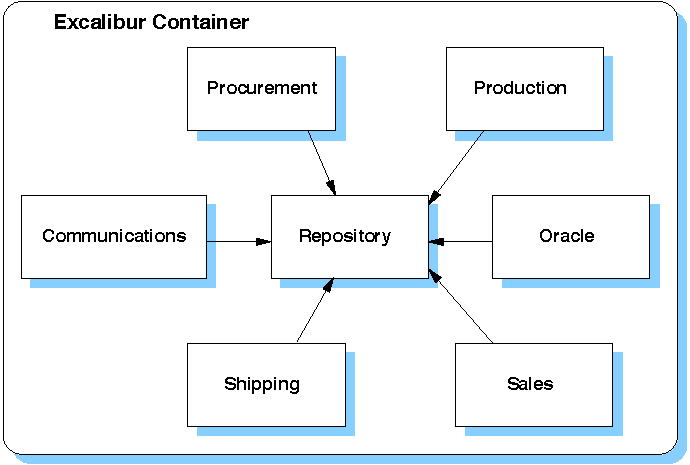
\includegraphics[width=0.7\textwidth]{figures/arch}
\caption{\label{fig:arch}MinneTAC architecture.  Arrows indicate dependencies.}
\end{figure}

Since decision components cannot depend on one another, they communicate using \emph{evaluations} that are accessible through the various data elements in the \textsc{Repository}.
Any calculations or analyses that are performed on \textsc{Repository} data can be encapsulated in the form of evaluations and made available to all other components via the \textsc{Repository}.
The \textsc{Oracle} component contains a large number of configurable \emph{evaluator} classes that perform analyses on \textsc{Repository} data.

All the major data elements in the \textsc{Repository}, such as RFQs, offers, components, and so forth, are Evaluable types.
Each Evaluable can be queried for related Evaluations by passing it the name of the needed evaluation.
An EvaluationFactory maintains a mapping of Evaluation names to Evaluator instances, and calls upon Evaluators to produce Evaluations on demand.
Evaluators can back-chain by requesting other Evaluations as they attempt to produce their results.
By this means an Evaluation may be composed from several other Evaluations that are in turn generated by their own Evaluators.

The resulting \textsc{Oracle} component is essentially a framework for a set of small, configurable sub-components from which other components can request analyses and predictions.
Most of these sub-components are Evaluators, though other types also exist.
The \textsc{Oracle} itself merely uses its configuration data to create and configure instances of Evaluators and other subclasses of ConfiguredObject.
\emph{ConfiguredObject} is an abstract class whose instances have names and some ability to configure themselves, given an appropriate clause from a XML configuration file.
The \textsc{Oracle} creates ConfiguredObject instances and keeps track of them by mapping their names as given in the configuration file to instances.

\begin{figure}[ht]
\centering
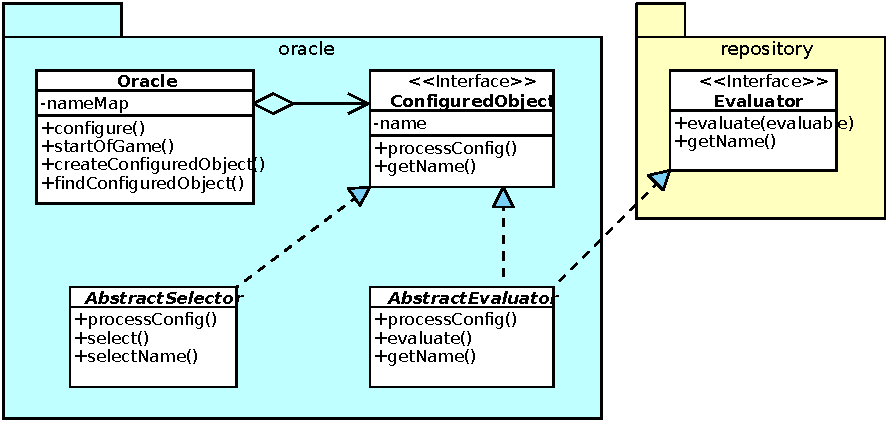
\includegraphics[width=\textwidth]{figures/oracle-classes}
\caption{Principal classes in the \textsc{Oracle} component}
\end{figure}

During initialization, the \textsc{Oracle} processes a configuration clause that specifies which ConfiguredObject instances to create, and for each such instance, what name to give it, the values of any parameters necessary to configure it, and the names of any instances it queries for input data.
Code listing~\ref{lst:xconf-simpleprice} illustrates such a configuration clause for an Evaluator with one parameter and four inputs.

{\small
\begin{lstlisting}[language={XML},frame={single},
label={lst:xconf-simpleprice},caption={Configuration clause for a price
evaluator that uses one parameter and several inputs}]
<evaluator
    class="edu.umn.cs.tac.oracle.eval.SimplePriceEvaluator"
    name="simple-price">
    <parameters price-probability-exponent="1.0"/>
</evaluator>
<graph source="simple-price">
    <quantity source="customer-quantity"/>
    <effective-demand source="effective-demand"/>
    <allocation source="allocation"/>
    <regression source="probability-of-acceptance"/>
</graph>
\end{lstlisting}
}

Taken together, a set of Evaluators and other ConfiguredObjects comprises a directed graph of modular components that constitute the majority of the functional code used in a MinneTAC agent workflow.
MinneTAC's modular architecture allows one to easily substitute components for one another for comparative purposes or to create an entirely new set of components with only minimal knowledge of how the agent works internally.
Additionally, using configuration files to define graphs of components allows developers to add new components without disrupting other developers' configurations.

\section{Usability challenges}
\label{sec:challenges}

MinneTAC Evaluators gather input data of specific types from zero or more other Evaluators, then use these data to produce one output of a given type.
In addition to having a specific set of inputs and outputs, Evaluators frequently have configuration parameters that affect how they behave.
Common parameters include exponents, probability thresholds, and more.
Creating an agent workflow involves choosing a set of Sink components from which the main decision-making components request data, choosing appropriate graphs of Evaluators that generate the data the chosen Sinks require, and finally configuring the individual Evaluators.~\cite{Collins08TR}

Historically, MinneTAC has proved itself difficult to configure because of how complex agent workflows, which tend to have graphs of over one hundred evaluators, tend to be.
Adding a component to a particular part of an agent workflow requires one to choose among hundreds of Evaluators, only a few of which are typically compatible with the relevant location in the workflow.
This makes the agent much less accessible to users who are less familiar with every available Evaluator.

Gil et al.~\cite{gil2010wings} identify another key issue that workflow designers face:  tracking and checking input and output constraints becomes onerous as the sizes of systems or the number of available components increase.
Manual workflow composition, as is the case with other user-driven tasks, is prone to errors and inconsistencies.

Maintaining input and output constraints while keeping the knowledge necessary to build and edit agent workflows to a reasonable level is a common problem in scientific workflow and service composition systems.
A number of existing technologies attempt to solve parts of this problem with a variety of methods for specifying and processing component metadata as well as choosing compatible components.
An informal survey of some of them reveals several common themes as well as important differences.

\subsection{Apache Excalibur}

Apache Excalibur\footnote{http://excalibur.apache.org/} is a general-purpose framework for building configurable systems out of independent components.
It is typically used as a foundation for server software and middleware, such a the Cocoon web application framework\footnote{http://cocoon.apache.org/}.
In the past MinneTAC used Excalibur extensively, so as a result MinneTAC's design is heavily influenced by Excalibur's architecture~\cite{Collins08ECRA}.
Excalibur components each fulfill specific \emph{roles}, while an Excalibur system is a set of roles, each realized by a class specified in a configuration file.

When starting, an Excalibur application reads configuration files that specify roles, classes that satisfy those roles, and configuration parameters for those classes.
The framework then instantiates the appropriate classes and invokes each component's interface.

Most of Excalibur's problems in this situation revolve around its extensive use of configuration files and framework methods for communications and inversion of control.
The configuration files often become exceedingly complex, increasing the likelihood of human error.
Information about what roles each component fills is kept exclusively within a configuration file that is separate from the component it represents.
When editing a system configuration one must cross-reference any changes made with component code and documentation, and vice versa --- changes to code must be reflected in system configurations.
Since role and configuration data are specified independently of the code, Excalibur requires that the programmer simply assert that they are consistent with one another; it performs no tests to determine if that is actually the case.
Moreover, even if metadata are specified correctly, code that uses the role metadata is not constrained to use them correctly.

\subsection{Enterprise JavaBeans 3.0 and the Spring Framework}
% Spring 2.x?

The Enterprise JavaBeans (EJB) specification\footnote{http://java.sun.com/products/ejb/} is one of several server-side Java EE APIs.
Before API version 3.0, JavaBeans applications were constructed similarly to Excalibur applications, via required interfaces and abstract classes specified by the API.
EJB gained a reputation for introducing complexity without delivering real benefits.

As a result, a counter-movement pushed for ``lighter-weight'' frameworks.
One of its products, the Spring Framework\footnote{http://www.springsource.org/}, is another open source application framework for Java and .NET applications.
Central to this framework is its Inversion of Control container, which provides a means of configuring and managing Java objects using callbacks, similar to Excalibur.
Where the Spring Framework differs from earlier versions of EJB is in how its component metadata are specified:  rather than using a configuration file or required API, one adds annotations to regular Java classes that specify which fields, methods, and classes need dependency injection.
The Spring Framework proved to be so successful that the EJB 3.0 specification borrowed so heavily from Spring that it was nearly completely rewritten.

Using source code annotations to supply component metadata links metadata with the code spatially.
This makes each component's metadata and code more likely to remain consistent than when they are specified in separate files, while still retaining the ability to take advantage of the metadata at runtime.
However, this method comes at the cost of static type checking --- systems built this way rely on programmers to assert that components implement the interfaces their annotations claim to support until such claims can be verified at runtime.

\subsection{WINGS}

The WINGS system proposed by Gil et al~\cite{gil2007wings} uses semantic component descriptions to help users create partial experiment workflows for the Pegasus workflow management service~\cite{callaghan2009scaling}.
Using an interactive editor one designs abstract versions of workflows that the workflow editor then fills in with concrete components and data sources using its knowledge base of component information.

This system successfully abstracts away the choice of components during the process of workflow design while still maintaining input and output constraints.
It is very flexible, allowing one to use nearly any sort of software as a component as long as one can describe it semantically.

Where WINGS falls short of our needs is its failure to link component semantics with component code; workflow authors simply have to trust that their component descriptions are accurate, and they do not learn about any disparities until runtime.
This is primarily a result of the system's design.
WINGS is a much more generalized system than we need that solves a subtly different problem, namely linking disparate applications together.
Since it needs to support software for which modifiable source may not be available it necessarily must support semantic descriptions that are decoupled from component code and cannot rely on internal annotations.

With MinneTAC we can benefit from a simpler, ``pipe-and-filter'' architecture that makes system design using semantics easier.
We can also benefit from access to component source code by employing methods that use Java annotations, which help link component code with their semantic descriptions.

\subsection{WSDL-S}

Rajasekaran et al~\cite{rajasekaran2005enhancing} proposed WSDL-S, an extension to the industry standard Web Services Description Language\footnote{http://www.w3.org/TR/wsdl20/}, an XML-based language that provides a model for describing web services.
WSDL-S adds semantic descriptions to the language that allows one to search for services based on their functional aspects rather than only by their names.
Using a rich description language both improves discoverability and reduces the chance of misinterpretation.

Since there is no all-encompassing standard for types in WSDL-S one has to provide some form of compatibility when describing a service's functionality to ensure clients are capable of interoperating correctly.
This can take any of several forms, the most common of which are using types that clients are assumed to understand, extending such a type and providing a downcasting operation, and creating a type and providing mappings to types that clients can recognize.
This makes it possible for WSDL-S to remain applicable to as wide a range of services as possible.

WSDL-S's companion tools, the Semantic Description Generator Module and METEOR-S~\cite{rajasekaran2005enhancing}, allow one to generate the semantic descriptions WSDL-S needs and provide an API for performing such queries.
These tools provide a way to spatially link operational code with semantic descriptions much like the Spring Framework, while retaining the generality of the WINGS system.
However, this suite fails to enforce coherence between semantic descriptions and their corresponding code, as they are specified independently of one another even though they may be located adjacent to one another.
We discuss our solution to this problem in section \ref{sec:approach}, where we describe our approach to applying semantic descriptions to the MinneTAC agent.

\section{Approach}
\label{sec:approach}

We aim to simplify MinneTAC's configuration process by creating a graphical editor for agent workflow configurations that draws upon ideas from Kim et al's Composition Analysis Tool~\cite{kim2004intelligent} as well as those from the systems surveyed in section \ref{sec:challenges}.
A graphical editor alone does nothing to fix the problem arising from the sheer number of Evaluators one has to choose from and thus be familiar with; at any point during workflow composition one may have to choose from a number of components when adding or replacing components.
By systematically generating a list of all of the valid choices throughout the workflow building process we can take context into account and only display Evaluators whose input or output data types are compatible with a given Evaluator.
This reduces the number of Evaluators users have to be familiar with at each step to only a small subset of all Evaluators, improving the chances that the agent will run correctly and making it simpler to write new components that are likely to work as intended.

\subsection{MinneTAC Ontology}

We accomplish this by creating a knowledge base of Evaluators and their input and output parameters using Web Ontology Language Description Logic (OWL-DL)\footnote{http://www.w3.org/TR/owl2-overview/}.
This semantic information allows us to query which Evaluators are compatible with one another's inputs and outputs.
Additionally, this gives us a way to programmatically check workflow configurations for consistency at configuration time rather than at runtime.

For this scheme to work one needs to define a \emph{component ontology} for each Evaluator that contains an ontological class describing its inputs and outputs.
These classes are unified by a top-level \emph{domain term ontology} that describes the data types used to represent inputs and outputs and their associated constraints.
The number of primitive types MinneTAC uses is small, consisting of about ten types, including prices, probabilities, and quantities.
We take advantage of this domain knowledge by placing only these primitive types in the domain term ontology and letting component ontologies define composite types on their own using templates for composite types that are also specified in the domain term ontology.
Simple OWL rules determine whether composite types specified by different component ontologies are compatible or not.
Employing our knowledge of the domain in this way solves a number of problems that typically plague workflow composition systems:

\begin{description}

\item[Workflows are easier to construct.]
As explained earlier, restricting the list of possible Evaluators one can add in the workflow editor to only those that make sense contextually makes each step in the workflow composition process faster since one only needs to compare a small number of Evaluators rather than sift through a long list of all Evaluators.

\item[Type incompatibilities are detected before runtime.]
Using annotations instead of interfaces comes at the cost of Java's static type checking, forcing workflow builders to prevent type incompatibilities on their own.
MinneTAC has this problem as well, but using semantics to restrict what choices are displayed in the workflow editor provides a degree of assurance that types are compatible at configuration time rather than at runtime.

\item[Evaluators are easy to annotate.]
Limiting the number of top-level domain types to be aware of makes it simple to find the correct types to assign to input and output annotations.

\item[Chances of evaluator duplication are reduced.]
If developers fail to immediately find Evaluators that do what they want while composing workflows they might create redundant ones, even if doing so means duplication, because writing new Evaluators is less of a cognitive burden than remembering them all.
A workflow editor that restricts the choices presented at each step increases the visibility of existing Evaluators that are contextually sensible.

\item[Chances of type duplication are reduced.]
The writer of a new Evaluator must choose the correct data types for its inputs and outputs.
When the domain term ontology is very large the most appropriate type might be overlooked, causing the writer to add a new, redundant type to it.
Keeping the number of types small reduces the likelihood of this problem.

\end{description}

The choice of size for the domain term ontology represents an important tradeoff between specificity and usability.
A small domain term ontology affords easier usability in that there are few types to learn when trying to assign input and output types to new Evaluators.
However, as they are few in number, these types are necessarily more generic than those from a larger domain term ontology, leading to ambiguity.
If domain types are too generic then so many Evaluators will match queries against their ontologies that the lists of valid Evaluators fail to be trimmed down to understandable levels.
This at least partially negates the benefit of using a workflow editor that makes use of semantic information.

However, opting toward a larger domain term ontology makes it difficult to choose the correct type out of the plethora of types that already exist when writing a new Evaluator.
In such a situation it may be easier to add still more new domain types than to decide whether any existing types are specific enough.
This reduces the utility of the workflow editor in the opposite way:  reasonable options may be overlooked.
For instance, this is a problem for some service-oriented applications like those that use Web Services Description Language (WSDL)~\footnote{http://www.w3.org/TR/wsdl20/}.
While semantic discovery systems like WSDL-S~\cite{rajasekaran2005enhancing} help alleviate problems specific to naming, the semantic descriptions such systems use rely on lists of types and other tag values for which there is no standardization.
Thus services are free to define their own, differing notations for the same purposes, creating duplication and limiting the utility of semantic searches.
Where the proper balance between larger, more specific domain term ontologies and smaller, more understandable domain term ontologies depends heavily on the domain in question.

\subsection{Using domain type information}

To fill out the component ontology we need to define an ontological class for each Evaluator.
With our previous code base this was impossible to do programmatically because Java only had knowledge of the native data types each Evaluator used, as opposed to the more specific domain data types needed to build OWL classes.
For instance, an array of \texttt{double} values indexed by \texttt{integer} values could represent anything from prices indexed by product IDs to probabilities indexed by lead times.
Domain information was specified solely in the documentation, making creating these classes a strictly manual process.
Each Evaluator thus had information about its input and output data types defined separately in five locations that had to be kept consistent manually:  its documentation, its ontology, its configuration code, its core logic, and in system configurations.
As a result, these tended to diverge from one another over time as they were not kept consistent automatically.
Using annotations to specify domain data types lets us use the same source of type information for each of these purposes.

An input annotation contains two main fields:  a name and a type declaration.
The name defines what name an Evaluator uses to request its input data from the \textsc{Repository}.
In the configuration file this name corresponds to the tag names in \texttt{graph} elements such as the one in code listing \ref{lst:xconf-simpleprice}.
The type declaration is a string containing any of the small number of scalar data types that makes up MinneTAC's domain term ontology or arrays thereof.
For example, a simple input annotation of scalar type might look like the following:

{\small
\begin{lstlisting}[language={Java},frame={single},label={lst:input-scalar},caption={An Input annotation with scalar type}]
@Input(name="probability", type="ProbabilityReal")
double probability;
\end{lstlisting}
}

When the workflow editor starts it loads each available Evaluator, creates an OWL class for it, and associates with this class an Input for each field it can find that has an Input annotation.
The field carrying the annotation in listing \ref{lst:input-scalar} ends up being represented by an Input of the scalar type ProbabilityReal, which is defined in the domain term ontology.

Non-scalar types are composed of scalar types from the domain term ontology.
When parsing a type of this sort the workflow editor creates a new subclass of types \texttt{1DArray}, \texttt{2DArray}, or so forth in the ontology and assigns cell types and index types to the subclass.
Simple OWL rules determine whether or not composite types defined by different components are equivalent to one another.
A two-dimensional array, for example, may have cells that contain product quotas which are indexed first by product ID and second by lead time.
An annotation for this may appear like the following:

{\small
\begin{lstlisting}[language={Java},frame={single},label={lst:input-composite},caption={An Input annotation with composite type}]
@Input(name="quota",
       type="QuantityReal[ProductIndex][LeadTimeInteger]")
double[][] quota;
\end{lstlisting}
}

Listing \ref{lst:input-composite} is an example of where we chose to use a simple type over several specific types.
We refer to product quotas as Quantities rather than ProductQuotas to reduce the size of the domain term ontology.
While this means some of the candidate Evaluators the workflow editor displays will be incorrect, the list of candidate Evaluators is short enough that it remains well within human cognitive ability.
For this reason, documentation remains important.
Input and Output annotations accept \texttt{description} strings in addition to their names and types.
Placing descriptions inside the annotations instead of in Javadoc comments allows the descriptions to be available to the workflow editor, which can then display descriptions alongside Evaluators to eliminate confusion about inputs' and outputs' specific meanings.
Javadoc displays Input and Output annotations alongside their associated fields and methods, so components' documentation is always consistent with their ontologies.

Output methods specify their return types with annotations in much the same way as inputs.
The workflow editor reads these as well and associates outputs with Evaluator classes in the component ontology.

{\small
\begin{lstlisting}[language={Java},frame={single},label={lst:output},caption={An Output annotation}]
  @Output(type="PriceReal[ProductIndex]")
  public Evaluation evaluate(Evaluable);
\end{lstlisting}
}

After creating OWL classes for each Evaluator, the workflow editor can query the component ontology to determine which Evaluator types are compatible with a given input or output type and only display those to the user composing the agent workflow.
An example of such a query's result appears in appendix \ref{sec:ontology-query}.

\subsection{Automatic input gathering}

In the past Evaluators had to individually devote code to reading their own configuration and input data.
This is because evaluators have individualized sets of inputs, making the code for fetching input data difficult to factor out.
As a result, many evaluators contain duplicate input-fetching code that often dwarfs their core logic in size.
One might find a given evaluator using any of several generations of input-gathering APIs or possibly even processing its own configuration clauses.
However, with input and configuration parameter variables now annotated with their domain data types this is no longer the case.
Since input fields are annotated as such a superclass method can reflectively find them, retrieve their values from the Evaluators named by the corresponding tags in the configuration file, and update their values.
As a result, while one annotates Evaluators to make them work with the MinneTAC ontology generator one can also replace nearly all of their input-reading code with a function call to a superclass method that does the same job.
This both improves serviceability and reduces the amount of boilerplate code necessary to write Evaluators.

To make use of this, variables used for input data must be class member fields rather than procedure-local variables so they can be accessed reflectively.
The superclass procedure, \emph{\texttt{populateInputs}}, then loops through the calling Evaluator's fields and retrieves the current value for any that have Input annotations using the same back end Evaluators formerly called directly.
An Evaluator need only call this method before it begins its computations.

For example, the Evaluator in Appendix \ref{sec:unannotatedeval} calls an old API's \texttt{getInput} method once for each input, which ends up as a procedure-local variable.
To convert this to use the new input gathering API one moves these variables to the class member level, annotates them with name and type information, then calls \texttt{populateInputs} in the location input values were previously read.

We can further reduce the amount of boilerplate code by applying the same procedure to Evaluator configuration parameters.
While parameters do not contribute to the workflow composition problem, they are still necessary for usability, as they must appear in the agent workflow editor.
Similarly to input gathering, calls to \texttt{getStringParameter} or similar procedures are replaced with a single call to \emph{\texttt{populateParameters}}.
Unlike inputs, parameters remain constant throughout the entire game, so one typically calls \texttt{populateParameters} at Evaluator construction time.

Updating the Evaluator from appendix \ref{sec:unannotatedeval} to use these annotation-based APIs yields the modified Evaluator shown in appendix \ref{sec:annotatedeval}.

Using input and output annotations in this way is the final step in consolidating type information.
When using the annotation-based API to gather input, Evaluators' input-gathering code is linked to annotations and no longer written separately.
This also constrains Evaluators' core logic to using inputs of the types given in annotations.
The \texttt{populateInputs} procedure call provides a point at which to do runtime type checking to provide additional enforcement of input and output constraints.
When we constrain Evaluators to using only types given by their semantic descriptions we eliminate one of the most serious problems with systems that use semantics:  having component code that does not match its semantic description.

\section{Conclusions and future work}

One major limitation of our current design is that it supports only one output type per Evaluator.
While this is sufficient for most Evaluators, in some cases it is better for an Evaluator to be capable of returning different results in certain contexts, such as when requesting information about specific products.
One possible way of alleviating this problem is allowing outputs to carry names in the same way as inputs.
Evaluators that wish to use outputs other than the default, unnamed output from other Evaluators may then specify which output name to use in the agent workflow configuration file.

In their current forms, input and output type annotations are specified by strings with a specific syntax (e.g., ``QuantityReal[ProductID]'').
This makes semantic description generators have to parse formatted text to discern which types annotations refer to.
We may be able to simplify this process by specifying array cell types and index types as separate attributes to Input and Output annotations.

TODO:  write a quick summary and maybe a little about our contributions (probably after working out what the Introduction section should say)

\section*{Acknowledgements}

TODO

\clearpage
\bibliographystyle{plain}
\bibliography{annotations2010}

\clearpage
\appendix

\section{Code listings}

\subsection{Un-annotated Evaluator example}
\label{sec:unannotatedeval}

{\small
\begin{lstlisting}[language={Java}]
public class SimplePriceEvaluator extends AbstractEvaluator
{
  private double probExponent = 1.0;

  public SimplePriceEvaluator(Repository rep,
                              Configuration config,
                              Logger logger) {
    super();
    init(rep, config, logger, "Revision:5673");
    getParameterValues();
  }

  private void getParameterValues() {
    probExponent = getDoubleParameter("price-probability-exponent",
                                      probExponent);
    addDependency("quantity",
                  getStringParameter("quantity-source", null));
    addDependency("allocation",
                  getStringParameter("allocation-source", null));
    addDependency("regression",
                  getStringParameter("regression-source", null));
    addDependency("effective-demand",
                  getStringParameter("effective-demand-source", null));
  }

  public Evaluation evaluate(Evaluable thing) {
    recomputeIfNecessary();
    // ...
  }

  private void recomputeIfNecessary() {
    // ...
    // Input gathering code
    // All local variables below are inputs.

    int[] actualDemand = null;
    double[] effectiveDemand
        = (double[])getInput(bom, "effective-demand");
    actualDemand = (int[])getInput(bom, "quantity");
    double[][] allocations = (double[][])getInput(bom, "allocation");
    Pricer[] poa = (Pricer[])getInput(bom, "regression");

    // ...
  }
}
\end{lstlisting}
}

\clearpage
\subsection{Annotated Evaluator example}
\label{sec:annotatedeval}

{\small
\begin{lstlisting}[language={Java}]
public class SimplePriceEvaluator extends AbstractEvaluator
{
  @Parameter(name="price-probability-exponent", defaultValue="1.0",
             description = "...")
  private double probExponent;

  @Input(name="quantity", type="QuantityInteger[ProductIndex]",
         required=false, description="...")
  private int[] actualDemand;

  @Input(name="effective-demand", type="QuantityReal[ProductIndex]",
         required=false, description="...")
  private double[] effectiveDemand;

  @Input(name="allocation", type="QuantityReal[ProductIndex][LeadTimeInteger]",
         description="...")
  private double[][] allocations;

  @Input(name="regression", type="Pricer[ProductIndex]", description="...")
  private Pricer[] poa;

  public SimplePriceEvaluator(Repository rep,
                              Configuration config,
                              Logger logger) {
    super();
    init(rep, config, logger, "Revision:6347");
    populateParameters();
  }

  @Output(type="PriceReal[ProductIndex]", description="...")
  public Evaluation evaluate(Evaluable thing) {
    recomputeIfNecessary();
    // ...
  }

  private void recomputeIfNecessary() {
    // ...
    // Input gathering code
    // All member variables that correspond to inputs are populated below.

    populateInputs();

    // ...
  }
}
\end{lstlisting}
}

\clearpage
\section{Ontology query example}
\label{sec:ontology-query}

This example shows the results of a query for compatible inputs and outputs for an EffectiveDemand data type.
The ``Superclasses'' and ``Usage'' sections indicate that EffectiveDemand is a valid input type for a SimplePriceEvaluator and a valid output for an EffectiveDemandEvaluator.

\subsection*{Asserted class hierarchy}

\begin{itemize}
\renewcommand{\labelitemi}{$\bullet$}
\renewcommand{\labelitemii}{$\bullet$}
\renewcommand{\labelitemiii}{$\bullet$}
    \item Thing
    \begin{itemize}
    \item Input\_Output
        \begin{itemize}
        \item EffectiveDemand
        \end{itemize}
    \end{itemize}
\end{itemize}

\subsection*{Superclasses}

\begin{itemize}
\item Input\_Output
\item hasDataType some QuantityArray
\item \emph{isInputOf some SimplePriceEvaluator}
\item \emph{isOutputOf some SimplePriceEvaluator}
\end{itemize}

\subsection*{Disjoints}

ed1\_out, sp1\_in

\subsection*{Usage}

\begin{itemize}
\item ed1\_out: EffectiveDemand
\item sp1\_in: EffectiveDemand
\item \emph{SimplePriceEvaluator $\subseteq$ hasInput some EffectiveDemand}
\end{itemize}

\end{document}
